\documentclass[12pt, fleqn, openany]{studyGuide}
\setstretch{1.4}
\enableInlineReview
\renewcommand{\VMBookTitle}{Audit Review}
\renewcommand{\VMBookSubtitle}{Grade 7 --- Ch Graphic Review --- Changed Questions}
\renewcommand{\VMFooterURL}{https://viewmath.com/grade7}
\renewcommand{\VMFooterURLDisplay}{ViewMath.com/Grade7}
\begin{document}

\begin{center}
\begin{tcolorbox}[
	enhanced,
	colback=white,
	colframe=funTeal!60,
	boxrule=1.5pt,
	arc=10pt,
	outer arc=10pt,
	width=0.9\linewidth,
	halign=center,
	top=5mm, bottom=5mm,
]
	{\Large\bfseries\sffamily\color{funTealDark}Audit Review}\\[2mm]
	{\large\sffamily\color{funGrayDark}Grade 7 --- Ch Graphic Review --- Changed Questions}\\[2mm]
	{\normalsize\sffamily\color{funGrayDark}Verify corrections below}
\end{tcolorbox}
\end{center}

\newpage
\section*{6-6-q23 \hfill \normalsize\texttt{tests\_questions\_bank\_2/topics/ch06-06-angle-relationships.tex}}
\begin{practiceQuestion}{6-6-q23}{gmc}
\begin{questionText}
In the figure below, $\angle AOB$ and $\angle BOC$ are complementary. Find the value of $x$.

\begin{center}
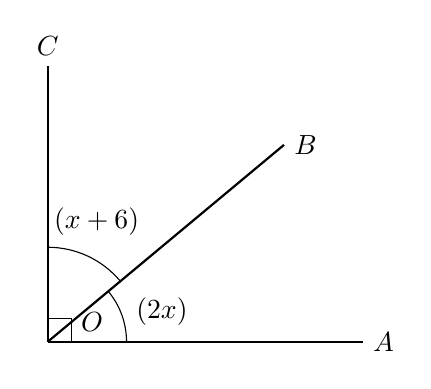
\begin{tikzpicture}[scale=1.0]
  \draw[thick] (0,0) -- (4,0) node[right] {$A$};
  \draw[thick] (0,0) -- (3,2.5) node[right] {$B$};
  \draw[thick] (0,0) -- (0,3.5) node[above] {$C$};
  \node at (0.3,0) [above right] {$O$};
  % Angle AOB
  \draw (1,0) arc[start angle=0,end angle=40,radius=1];
  \node at (1.45,0.38) {$(2x)°$};
  % Angle BOC
  \draw (0,1.2) arc[start angle=90,end angle=40,radius=1.2];
  \node at (0.62,1.52) {$(x+6)°$};
  % Right angle mark
  \draw (0.3,0) -- (0.3,0.3) -- (0,0.3);
\end{tikzpicture}
\end{center}
\end{questionText}
\choiceA{$24$}
\choiceB{$28$}
\choiceC{$32$}
\choiceD{$36$}
\correctAnswer{B}
\explanation{Since $\angle AOC = 90°$, the two angles are complementary: $2x + (x + 6) = 90$. Combine: $3x + 6 = 90$. Subtract $6$: $3x = 84$. Divide: $x = 28$.}
\end{practiceQuestion}

\newpage
\section*{m-6-6-q24 \hfill \normalsize\texttt{tests\_questions\_bank\_2/topics\_modified/ch06-06-angle-relationships.tex}}
\begin{practiceQuestion}{m-6-6-q24}{gmc}
\begin{questionText}
In the triangle below, an exterior angle is formed at vertex $C$. Find the measure of the exterior angle.

\begin{center}
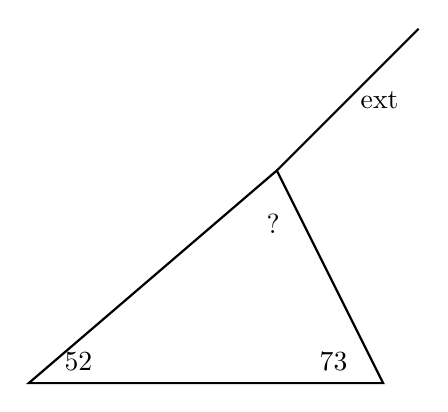
\begin{tikzpicture}[scale=0.9]
  \coordinate (A) at (0,0);
  \coordinate (B) at (5,0);
  \coordinate (C) at (3.5,3);
  \draw[thick] (A) -- (B) -- (C) -- cycle;
  % Exterior angle at C
  \draw[thick] (C) -- (5.5,5);
  % Interior angles
  \node at (0.7,0.3) {$52°$};
  \node at (4.3,0.3) {$73°$};
  \node at (3.45,2.25) {$?$};
  % Exterior angle label
  \node at (4.95,4.0) {ext};
\end{tikzpicture}
\end{center}
\end{questionText}
\choiceA{$55°$}
\choiceB{$107°$}
\choiceC{$125°$}
\choiceD{$180°$}
\correctAnswer{C}
\explanation{The interior angle at $C$ is $180° - 52° - 73° = 55°$. The exterior angle is supplementary to the interior angle at $C$: $180° - 55° = 125°$. Alternatively, by the exterior angle theorem: $52° + 73° = 125°$.}
\end{practiceQuestion}

\newpage
\section*{m-6-6-q27 \hfill \normalsize\texttt{tests\_questions\_bank\_2/topics\_modified/ch06-06-angle-relationships.tex}}
\begin{practiceQuestion}{m-6-6-q27}{gsa}
\begin{questionText}
In the diagram, $\triangle ABC$ is shown with an exterior angle at $B$. $\angle A = (3x + 5)°$ and $\angle C = (2x + 15)°$. The exterior angle at $B$ is $(7x - 10)°$. Find $x$ and all angle measures.

\begin{center}
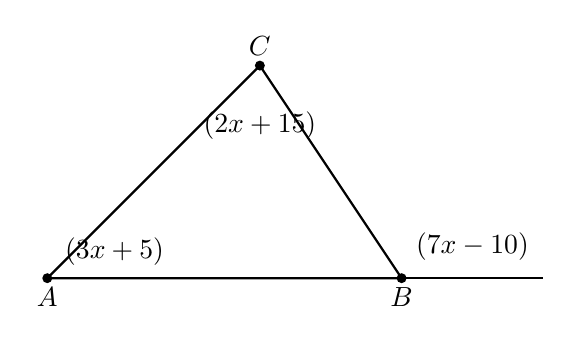
\begin{tikzpicture}[scale=0.9]
  \coordinate (A) at (0,0);
  \coordinate (B) at (5,0);
  \coordinate (C) at (3,3);
  \draw[thick] (A) -- (B) -- (C) -- cycle;
  % Exterior angle at B
  \draw[thick] (B) -- (7,0);
  % Labels
  \node at (0.95,0.38) {$(3x+5)°$};
  \node at (3.0,2.15) {$(2x+15)°$};
  \node at (6.0,0.45) {$(7x-10)°$};
  \fill (A) circle (2pt) node[below] {$A$};
  \fill (B) circle (2pt) node[below] {$B$};
  \fill (C) circle (2pt) node[above] {$C$};
\end{tikzpicture}
\end{center}
\end{questionText}
\correctAnswer{$x = 15$; $\angle A = 50°$, $\angle C = 45°$, $\angle B = 85°$, exterior angle $= 95°$}
\explanation{By the exterior angle theorem, the exterior angle equals the sum of the two non-adjacent interior angles: $7x - 10 = (3x + 5) + (2x + 15)$. Simplify: $7x - 10 = 5x + 20$. Subtract $5x$: $2x - 10 = 20$. Add $10$: $2x = 30$. Divide: $x = 15$. Then $\angle A = 3(15) + 5 = 50°$, $\angle C = 2(15) + 15 = 45°$. Interior $\angle B = 180° - 50° - 45° = 85°$. Exterior angle $= 7(15) - 10 = 95°$. Verify: $50 + 45 = 95$ \checkmark.}
\end{practiceQuestion}

\end{document}